
\begin{dialog}{音程增值的卡农}

\begin{quote}
阿基里斯和乌龟刚刚在城里最好的中餐馆吃过一顿美味的中餐。
\end{quote}

\begin{dialogue}

\item[阿基里斯]你筷子使得挺溜儿,龟兄。

\item[乌龟]那很自然。我打年轻时起就喜欢东方菜,你呢——你这顿饭吃得好吗,阿基?

\item[阿基里斯]非常好。以前我从没吃过中餐。这顿饭是个极好的开端。你现在着急走吗?我们就坐在这儿聊会儿怎么样?

\item[乌龟]我喜欢边喝茶边聊。喂,伙计!

\dnote{(一位侍者走过来。)}

请把帐单拿给我们,再来些茶。

\dnote{(侍者急匆匆地离开了。)}

\item[阿基里斯]在中式烹饪方面你比我知道得多,龟兄,可是在日本诗歌方面,我敢打赌我比你知道得多。你读过俳句吗?

\item[乌龟]恐怕没读过。什么是俳句?

\item[阿基里斯]俳句是一种由十七个音节组成的日本诗——更确切地说是种微型诗。也许它就像馥郁芳香的玫瑰花瓣或蒙蒙细雨中的百合塘一样容易叫人产生联想。它通常由五个音节、七个音节、再五个音节这样三部分组成。

\item[乌龟]诗这么简短,只有十七个音节,意义不会多……

\item[阿基里斯]意义很深远,半在读者心中存,半在俳句中。

\item[乌龟]嗯……这是种容易叫人产生联想的表达方法。\dlnote{(侍者拿着帐单、一壶茶和两个福气小甜饼走过来。)}

谢谢,伙计。再加点茶吧,阿基?

\item[阿基里斯]好吧。这些小甜饼看来很好吃。\dlnote{(拿起一个,咬了一口,嚼了起来。)}嘿!这里面是什么怪玩意?一张小纸片?

\item[乌龟]那是你的福签,阿基。许多美国的中餐馆结账的时候都把福气小甜饼和帐单一起送来,起联络顾客感情的作用。要是你经常出入中餐馆的话,你就会把福气小甜饼更多地看作消息的传递者,而不仅仅把它当做小甜饼。可惜的是你似乎已经把你的福气吞掉一部分了。剩下那部分说些什么?

\item[阿基里斯]有点怪啊,所有的字都紧密地排在一起,彼此之间没有空隙。也许这需要用某种方法来破译?噢,现在我明白了。如果你把空隙放回它们原来该在的地方,即是:“{\ziju{1}禾灿邻晴}”。我真觉得没头没脑的。也许它是首俳句式的诗,我把大部分的字都吃掉了。

\item[乌龟]那样一来,你现在的福签就只是俳句的$4/17$了。它唤起的意象挺怪的。如果俳句的$4/17$是一种新的艺术形式,那我只好说:此事堪哀……不过,我可以瞧瞧它吗?

\item[阿基里斯]\dlnote{(把那块小纸片递給乌龟)}当然可以。

\item[乌龟]啊,要是让我来破译它,阿基,它就变得完全不一样了!它写的是“秋 岭 阳 青”。看来也许它原本是首很好的抒情俳句呢。

\item[阿基里斯]你说的对,它还挺有意境的。

\item[乌龟]我所做的只不过是把阅读框架移动了一个单位——就是说,我把所有的空隙向右移动了一个单位。

\item[阿基里斯]让我们来看看你的福签怎么说,龟兄。

\item[乌龟]\dlnote{(灵巧地掰开他的小甜饼,读道)}“福气很深远,半在食客手中托,半在甜饼中”。

\item[阿基里斯]你的福签也是一首俳句,龟兄——至少它采用了$5$-$7$-$5$共十七个字的形式。

\item[乌龟]太了不起了。阿基,我还真没注意到这一点。这种事只有你会注意。它更吸引我的地方还是它的内容——当然,它是可以解译的。

\item[阿基里斯]我认为这事表明我们每个人都各有自己的方法来解译我们所接受的信息……

\dnote{(一阵沉默,阿基里斯盯着空茶杯底上的茶叶。)}

\item[乌龟]再加些茶吗,阿基?

\item[阿基里斯]好的,谢谢。哎,龟兄,你那位朋友螃蟹怎么样了?自从你跟我说了你们那场奇特的唱机之战以后,我老是想起他。

\item[乌龟]我也跟他谈起过你,他很想见你。他近来很好。最近在唱机方面他又得到了一个新玩艺儿:一种少见的自动唱机。

\item[阿基里斯]哦,就是酒吧间里那种有许多用来选歌的按钮,投入硬币后就能自动放唱片的玩意儿吗?

\item[乌龟]对,可这架自动唱机太大了,他的屋子里都放不下,他只好在房子后面特地为它盖了一间小屋。

\item[阿基里斯]我无法想象它怎么会这么大,除非它里面装了许多唱片。是这样吗?

\item[乌龟]实际上它只有一张唱片。

\item[阿基里斯]什么?一架自动唱机只有一张唱片?自相矛盾。那么,这架自动唱机为什么会这么大?它那仅有的一张唱片十分巨大吗?——直径有十公尺?

\item[乌龟]不,它不过是一张普通的自动唱机上的唱片。

\item[阿基里斯]那么,龟兄,你一定是在戏弄我。说到底,什么样的自动唱机只能播出一首歌?

\item[乌龟]谁说就一首歌啦,阿基?

\item[阿基里斯]我所见过的所有自动唱机都遵循那条基本的自动唱机公理:“一张唱片一首歌。”

\item[乌龟]这架自动唱机可不一样,阿基。唱片垂直地悬挂着,在它后面有一个小巧的架空的轨道网,上面挂着各种各样的唱头。当你揿某一对按钮——比如说B-1——时,它就会选择那些唱头中的某一个。这样就触发了某个自动机构,使唱头沿着生锈的轨道吱吱地运行起来。直到最后它转到唱片附近——也就是说,进入了播放位置。

\item[阿基里斯]然后那张唱片开始旋转,同时播放出音乐来——对吗?

\item[乌龟]不太对。唱片不动——唱头旋转。

\item[阿基里斯]我本该想到的。可是,如果你只有一张唱片可放,这稀奇古怪的玩意怎么能播出不止一首歌呢?

\item[乌龟]这问题我问过螃蟹。他只是建议我来试验一下。于是我从口袋里掏出一枚五分硬币(用一枚五分硬币你可以选三首歌),把它塞进投币槽里,先揿动B-1按钮,然后是C-3、B-10——这全都是随意的。

\item[阿基里斯]那么,我想,B-1唱头滑入轨道后,咬住那张垂直的唱片,然后开始旋转?

\item[乌龟]没错儿。播放的那段音乐还是很动人的,它是根据有名的B-A-C-H旋律改编的,我相信你记得它……

  \begin{center}
  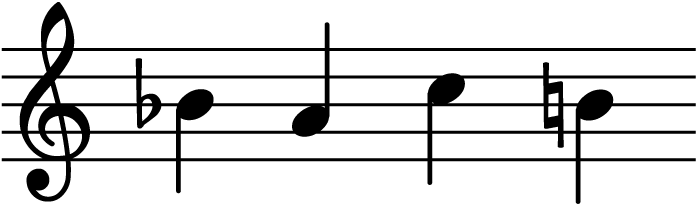
\includegraphics[width=.5\linewidth]{img_dialog06_1.png}
  \end{center}

\item[阿基里斯]我怎么会记不得呢?

\item[乌龟]这是B-1唱头。这支曲子结束后,它缓慢地转回它原来悬挂的位置,而C-3滑入了播放位置。

\item[阿基里斯]C-3是不是播出了另一支歌?

\item[乌龟]是这样。

\item[阿基里斯]啊,我明白了。它播出的是唱片反面的歌,要不就是同一面上的另一个音段。

\item[乌龟]不,这张唱片只有一面有音槽,而且只有那么一个音段。

\item[阿基里斯]我一点也不明白。你不可能用同一张唱片播放出许多不同的音乐!

\item[乌龟]在我看到老蟹的自动唱机之前,也是这么想。

\item[阿基里斯]那第二支歌怎么唱?

\item[乌龟]十分有趣……这是首根据C-A-G-E旋律改编成的歌。

  \begin{center}
  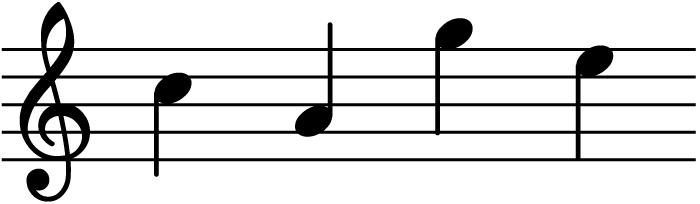
\includegraphics[width=.5\linewidth]{img_dialog06_2.png}
  \end{center}

\item[阿基里斯]这可是支全然不同的曲子啊!

\item[乌龟]千真万确。

\item[阿基里斯]约翰·卡奇[John Cage]不是个现代音乐作曲家吗?我好像记得在我的那些关于俳句的书中有一本谈到过他。

\item[乌龟]一点不错。他创作过很多著名的曲子,其中包括《4分33秒》,这是一部三个乐章的作品,由一些长度不等的静默组成,是极富于表现力的——如果你喜欢这一类东西的话。

\item[阿基里斯]我想我要是在一家喧声刺耳的咖啡馆里,肯定愿意出钱听自动唱机播放卡奇的《4分33秒》。它可以让人们平心静气!

\item[乌龟]是啊——谁想听盘碟碗筷发出的哗啦哗啦的噪音呢?啊,对啦,《4分33秒》还有一个用武之地:兵营。

\item[阿基里斯]你的意思是说让它去和大兵们穿的卡其布军装配套,是吗?嗯,我想这说得通。至于螃蟹的自动唱机……我就不明白了。“BACH”和“CAGE”怎么能同时编码于同一张唱片上呢?

\item[乌龟]如果你仔细研究研究它们,阿基,你会发现两者间存在着某种联系。让我说明一下:若是你把曲子“B-A-C-H”中各音的间距列出来,会得到什么呢?

\item[阿基里斯]让我想想。先降半音,从B降到A(这里B采用的是德国记谱法),然后再升三个半音,升到C;最后又降半音,降到H。这就得出下面的形式:
  \[
  -1, +3, -1
  \]
\item[乌龟]非常正确。那么,“C-A-G-E”呢?

\item[阿基里斯]在这里,开始先降三个半音,然后再升十个半音(几乎一个八度),最后再降三个半音。这就是说其形式是这样的:
  \[
  -3, +10, -3
  \]
  与前一个非常相像,不是吗?

\item[乌龟]的确是这样。在某种意义上,它们几乎有同样的“构架”。你可以通过把所有的音程乘上$3\frac13$,并取最近的整数,从B-A-C-H得到C-A-G-E。

\item[阿基里斯]嘿,真是令我又惊又喜!这意味着音纹中只有一种构架编码,而各种各样的唱头把它们自己对编码的解译加到了编码上,是吗?

\item[乌龟]确实不清楚。狡猾的螃蟹不愿让我知道详情。但是当唱头B-10转入播放位置时,我确实听到了第三支歌。

\item[阿基里斯]那歌怎么唱?

\item[乌龟]这支曲子由极宽的音程组成,它们是B-C-A-H:
  \begin{center}
  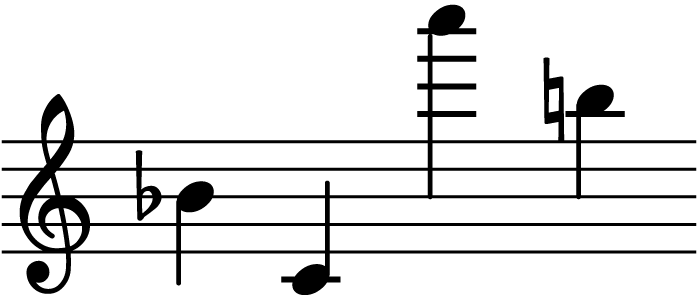
\includegraphics[width=.5\linewidth]{img_dialog06_3.png}
  \end{center}
  用半音计算,其音程形式是:
  \[
  -10, +33, -10
  \]
  它可以通过由CAGE再乘以$3\frac13$,并取最近的整数得到。

\item[阿基里斯]这种音程变换有什么名称吗?

\item[乌龟]人们都管它叫“音程增值”。它类似于卡农的时值增值,在那种增值里,一个旋律里所有音符的时值被某一常数相乘。在那里,结果只是使曲子慢下来;而在这里,结果是用某种奇特的方法扩展了旋律的音域。

\item[阿基里斯]有意思。那么你所试的三个旋律都是那张唱片上同一音纹模式的几个音程增值的形式,是吗?

\item[乌龟]这就是我得出的结论。

\item[阿基里斯]让我感到难以思议的是,当你增值巴赫[BACH]时,你得到卡奇[CAGE],而当你再增值卡奇[CAGE]时,你又回到巴赫[BCAH],只是里面两个字母的顺序颠倒了,好像巴赫在通过了卡奇这个中间阶段后有点反胃。
\item[乌龟]这听起来像是对卡奇的那种新艺术形式所作的有见地的评论。

\end{dialogue}

\end{dialog}
